\documentclass[../Article_Model_Parameters.tex]{subfiles}
\graphicspath{{\subfix{../Figures/}}}
\begin{document}
	
	A supercritical fluid (SCF) is a substance at a temperature and pressure above its critical point, where there are no distinct liquid and gas phases but below the pressure required to compress it into a solid. SCFs can move through porous solids like gases, which is faster than liquid transport through such materials. SCFs have a higher ability to dissolve materials like liquids or solids compared to gases. Near the critical point, small changes in pressure or temperature result in significant changes in density, allowing many properties of an SCF to be fine-tuned. By changing the pressure and temperature, the properties can be tuned to be more liquid-like or gas-like.
	
	Fluid properties can be divided into two kinds: equilibrium properties and transport properties. The equation of state can be used accurately to predict the equilibrium properties, such as density, enthalpy, vapour pressure, fugacity and fugacity coefficient, vapour-liquid equilibrium, and all kinds of excess properties.
	
	Supercritical $CO_2$'s thermodynamic properties, such as density, the local speed of sound, and specific heat capacity, vary significantly with slight changes in temperature and pressure due to real gas effects. The Peng-Robinson equation of state (P-R EOS) is used to calculate the thermodynamic properties by accounting for these real gas effects. The P-R EOS belongs to a specific class of thermodynamic models for modelling the pressure of a gas as a function of temperature and density. It can be written as a cubic function of the molar volume (of the density). Detail information about Peng-Robinson equation of state can be found in the work of \citet{Peng1976}, \citet{Elliott2011} or \citet{Pratt2001}. The P-R EOS is presented by Equation \ref{EQ: PR}
	
	{\footnotesize
		\begin{equation}
			P = \cfrac{RT}{V_m - b} - \cfrac{a\alpha}{V_m^2 + 2bV_m - b^2}
			\label{EQ: PR}
		\end{equation}
	}
	
	The parameters $a, b, \alpha$ are parameters defined as presented in the Appendix \ref{subsubsec: Equation of state}.
	
	The properties of $CO_2$  are presented as a function of operating conditions (temperature and pressure) in Figure \ref{fig: SFE_Properties}. At standard atmospheric pressure and temperature, $CO_2$  behaves as an ideal gas, and its compressibility factor equals unity. However, at high pressures and/or low temperatures, intermolecular forces between gas molecules become more significant, causing them to deviate from ideal behaviour. As a result, the compressibility factor can either be greater than or less than unity, depending on the magnitude of these forces. As presented in Figure \ref{fig: SFE_Properties_Compressibility}, the compressibility factor obtained from the Peng-Robinson equation of state varies strongly depending on the operating conditions. The compressibility factor can be obtained by solving the polynomial form of the P-R EOS given by Equation \ref{EQ: PR_polynomial}.
	
	{\footnotesize
		\begin{equation}
			Z^3 - (1-B)Z^2+(A-2B-3B^2)Z -(AB-B^2-B^3) = 0
			\label{EQ: PR_polynomial}
		\end{equation}
	}
	
	where $A$ and $B$ are parameters as defined in the Appendix \ref{subsubsec: Equation of state}. The roots of the polynomial can be found iteratively or by the Cardano formula. In a one-phase region, the fluid is described by one real root corresponding to the gas, liquid or supercritical phase. The gas-liquid mixture is present in the two-phase region, and two roots are found. The biggest root is assigned to the gas phase, and the smallest root corresponds to the liquid phase.
	
	The real gas effects are also visible on the density plot presented in Figure \ref{fig: SFE_Properties_Density}. The density calculations are based on the compressibility factor and its value depends on the operating conditions. The fluid's properties near the critical point are unique and combine gas-like and liquid-like properties. The details of calculations are explained in the Appendix \ref{subsubsec: Fluid density}.
	
	Figure \ref{fig: SFE_Properties_CP} show the behaviour of the heat capacity of a supercritical fluid at constant pressure ($C_p$). The details of the calculations can be found in the Appendix \ref{subsubsec: Fluid heat capacity}. Contrary to the density, which varies monotonically, the specific heat shows very high levels in a narrow region. In the subcritical region, the phase transition is associated with an effective spike in the heat capacity (i.e., the latent heat). Approaching the critical point, the latent heat falls to zero, which is accompanied by a gradual rise in heat capacity in the pure phases near phase transition. At the critical point, the latent heat is zero, but the heat capacity shows a diverging singularity. Beyond the critical point, there is no divergence, but rather a smooth peak in the heat capacity; the highest point of this peak identifies the Widom line (as discussed by \citet{Simeoni2010} and \citet{Banuti2019}).
	
	To determine the thermodynamic properties of a real gas, it is necessary to evaluate the departure function of the chosen equation of state for that property. As explained by \citet{Elliott2011}, the departure function is the difference between the actual value of a thermodynamic property of a real gas and its value if the gas were ideal under the same temperature and pressure conditions. The ideal gas serves as a reference state to which the properties of real gases are compared. The departure function is a measure of the extent to which a real gas deviates from ideal gas behaviour. The departure functions allow for the accurate calculation of thermodynamic properties for real gases.  %(10.1007/s10494-017-9872-4)
	
	\begin{figure*}[H]
		\begin{subfigure}[b]{0.95\textwidth}
			\centering
			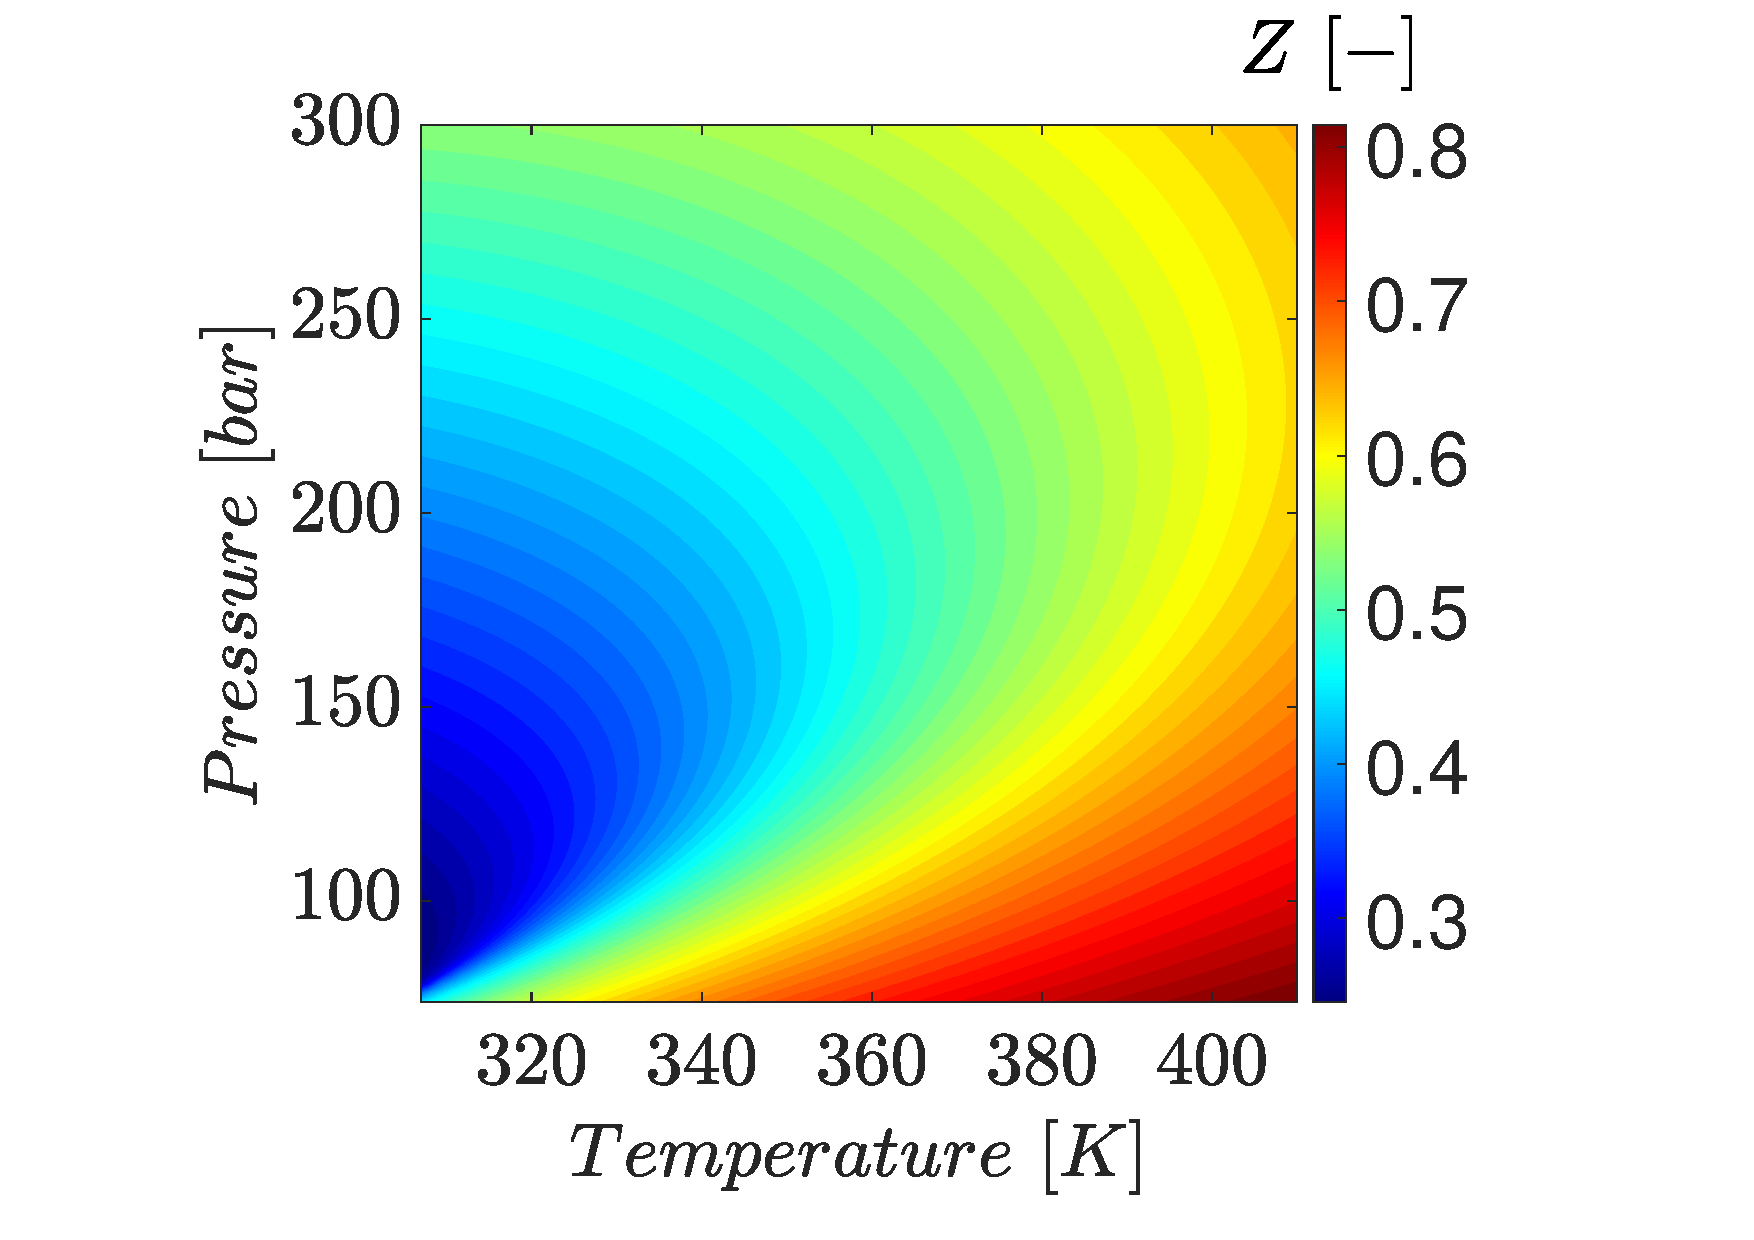
\includegraphics[trim = 2.9cm 7cm 3cm 7cm,clip,width=\textwidth]{Figures/Compressibility.pdf}	
			\caption{The compressibility factor based on the Peng-Robinson equation of state}
			\label{fig: SFE_Properties_Compressibility}
		\end{subfigure}
		\hfill
		\begin{subfigure}[b]{0.95\textwidth}
			\centering
			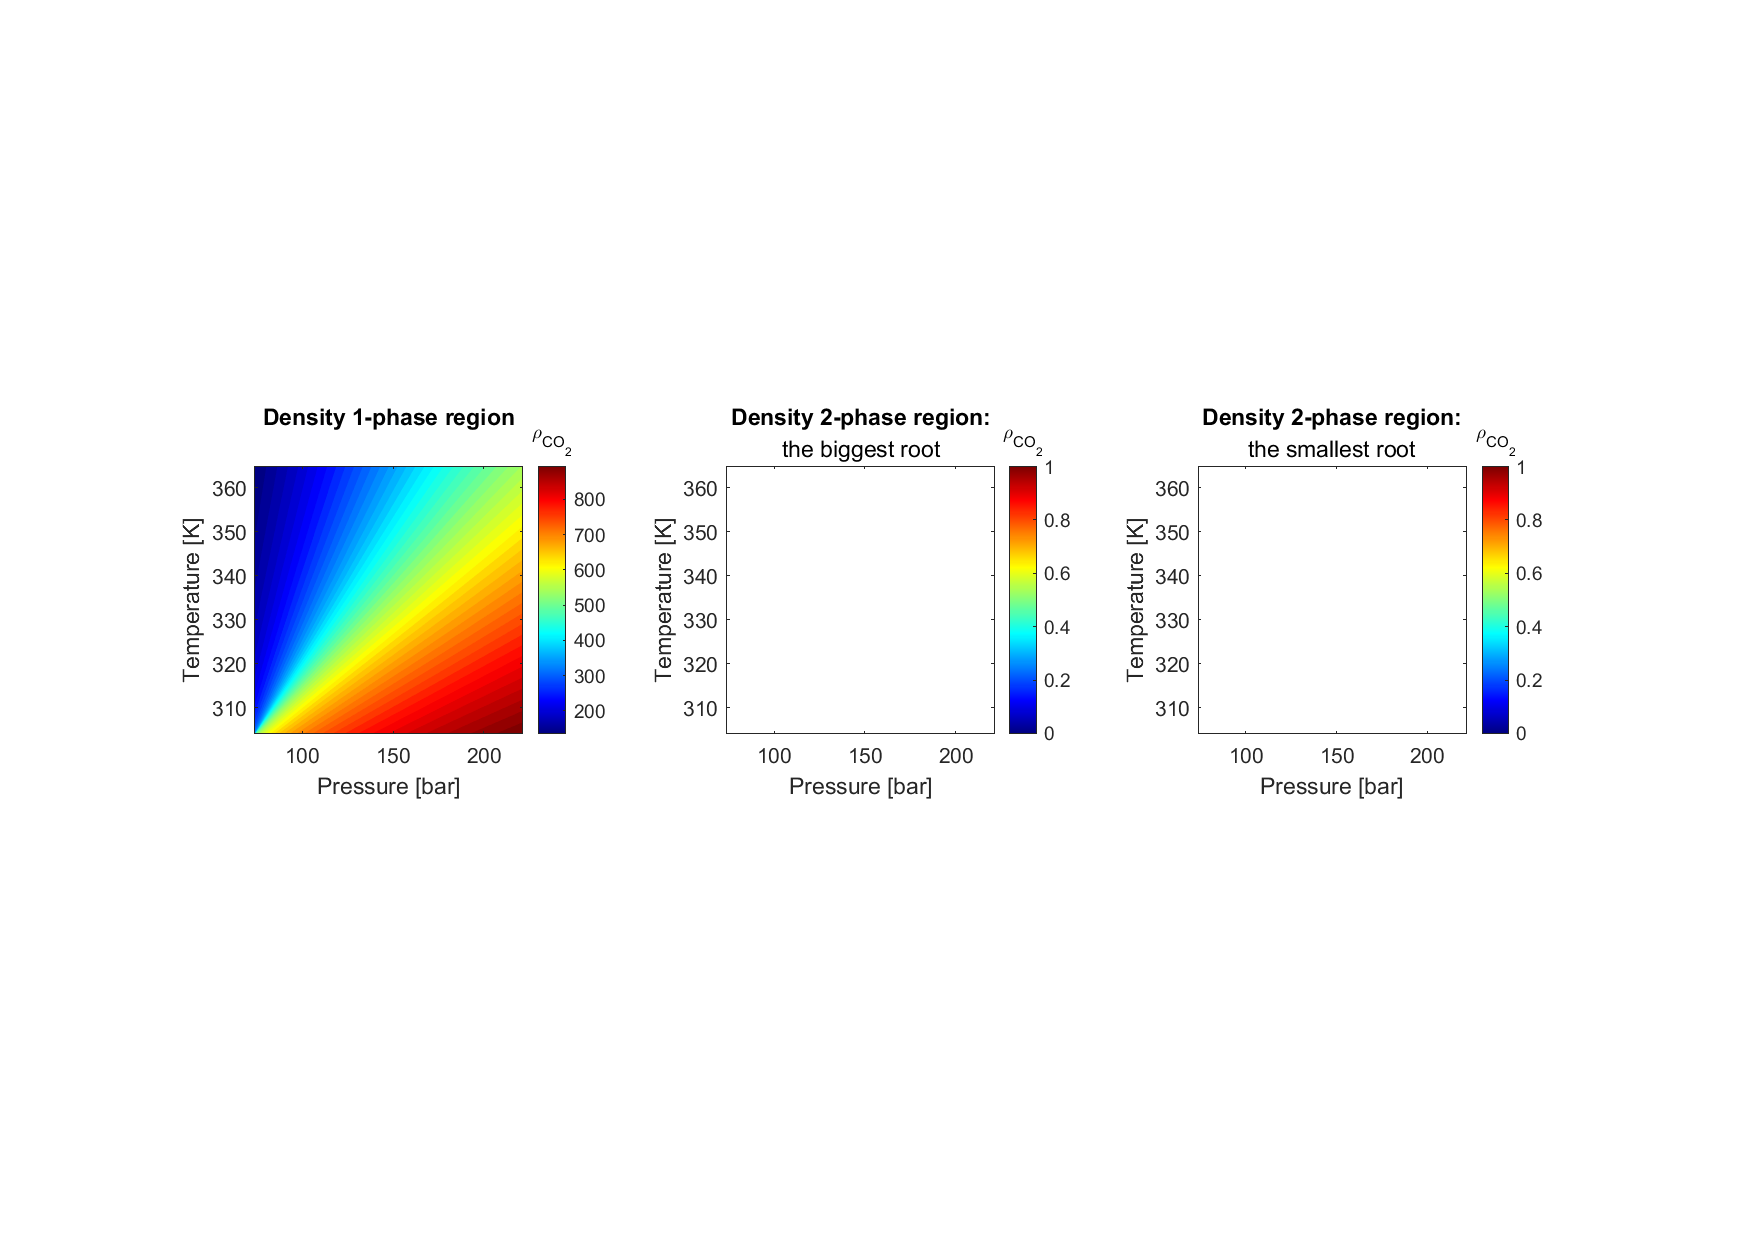
\includegraphics[trim = 2.9cm 7cm 3cm 7cm,clip,width=\textwidth]{Figures/RHO.pdf}	
			\caption{The fluid density based on the Peng-Robinson equation of state}
			\label{fig: SFE_Properties_Density}
		\end{subfigure}
		\hfill
		\begin{subfigure}[b]{0.95\textwidth}
			\centering
			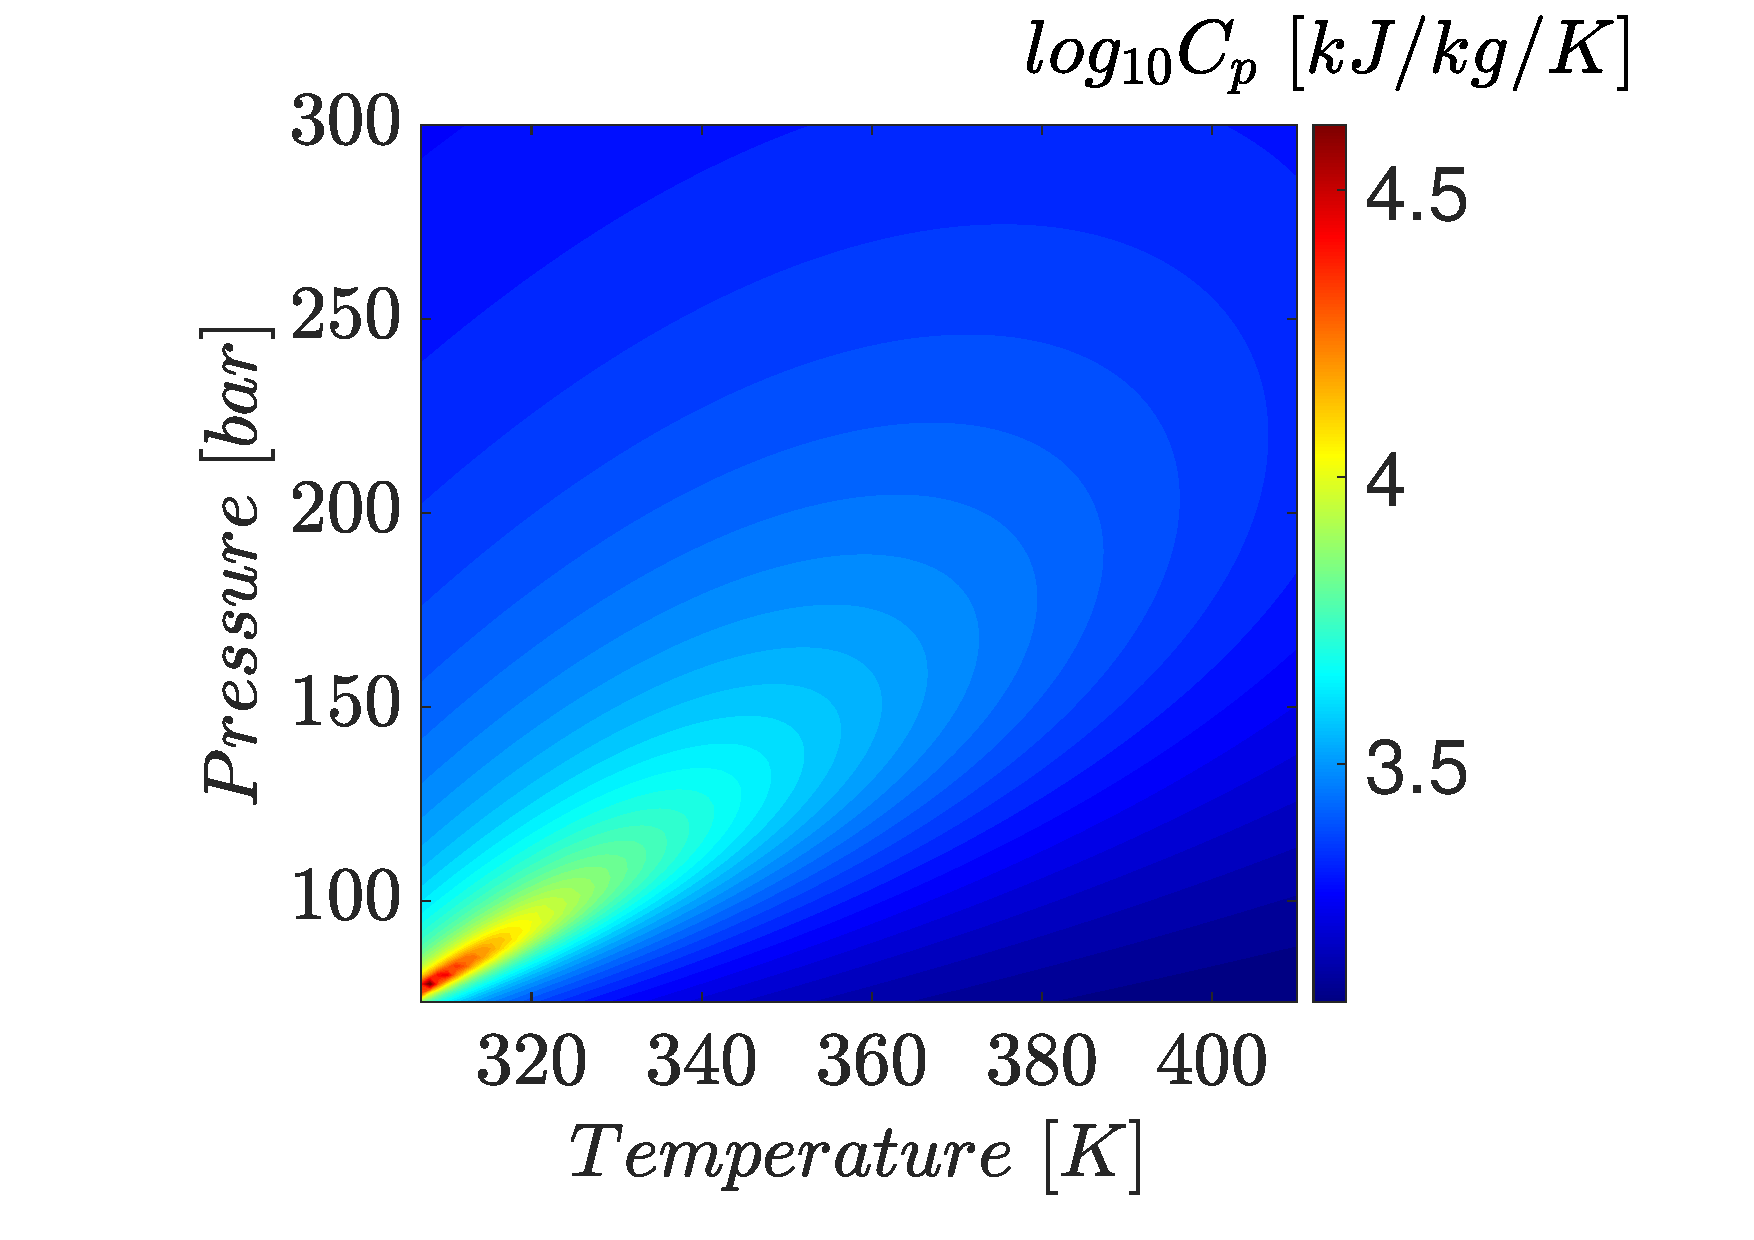
\includegraphics[trim = 2.9cm 7cm 3.cm 7cm,clip,width=\textwidth]{Figures/CP.pdf}	
			\caption{The specific heat of the $CO_2$ based on the Peng-Robinson equation of state}
			\label{fig: SFE_Properties_CP}
		\end{subfigure}
		\caption{Properties of $CO_2$ based on the equation of state}
		\label{fig: SFE_Properties}
	\end{figure*}    
	
	Transport properties such as viscosity and conductivity play a crucial role in engineering design for production, fluid transportation, and processing. However, as highlighted by \citet{Sheng1989}, developing a satisfactory theory for transport properties of real dense gases and liquids is a challenging task. This is due to the inherent difficulties involved in accurate measurements and the complexity involved in theoretical treatments.
	
	To address this issue, the correlations of transport coefficients are either empirical or based on some theoretical foundation. Chapman-Enskog's theory (presented in \citet{Chapman1991}) for transport properties of dense gases based on the distribution function is a popular theoretical approach. However, the Chapman-Enskog theory was developed for rigid spherical molecules and modifications are required to apply it to real gases. Many correlations have been proposed following the Chapman-Enskog theory in the form of reduced density and reduced temperature, such as those developed by \citet{Fenghour1998} and \citet{Laesecke2017} from the National Institute of Standards and Technology (NIST). A comparison of these correlations is presented in Figure \ref{fig: SFE_Properties_mu}.
	
	NIST has developed a viscosity formulation consisting of four contributions: (i) for the limit of zero density, (ii) for the initial density dependence, (iii) for the residual viscosity, and (iv) for the singularity of the viscosity at the critical point. The NIST correlation covers temperatures from 100 to 2000 $K$ for gaseous $CO_2$, and from 220 to 700 $K$ with pressures along the melting line up to 8000 $MPa$ for compressed and supercritical liquid states. These correlations and theories are essential in predicting transport properties for real gases and liquids and can assist in engineering design and analysis.
	
	\begin{figure*}[H]
		\centering
		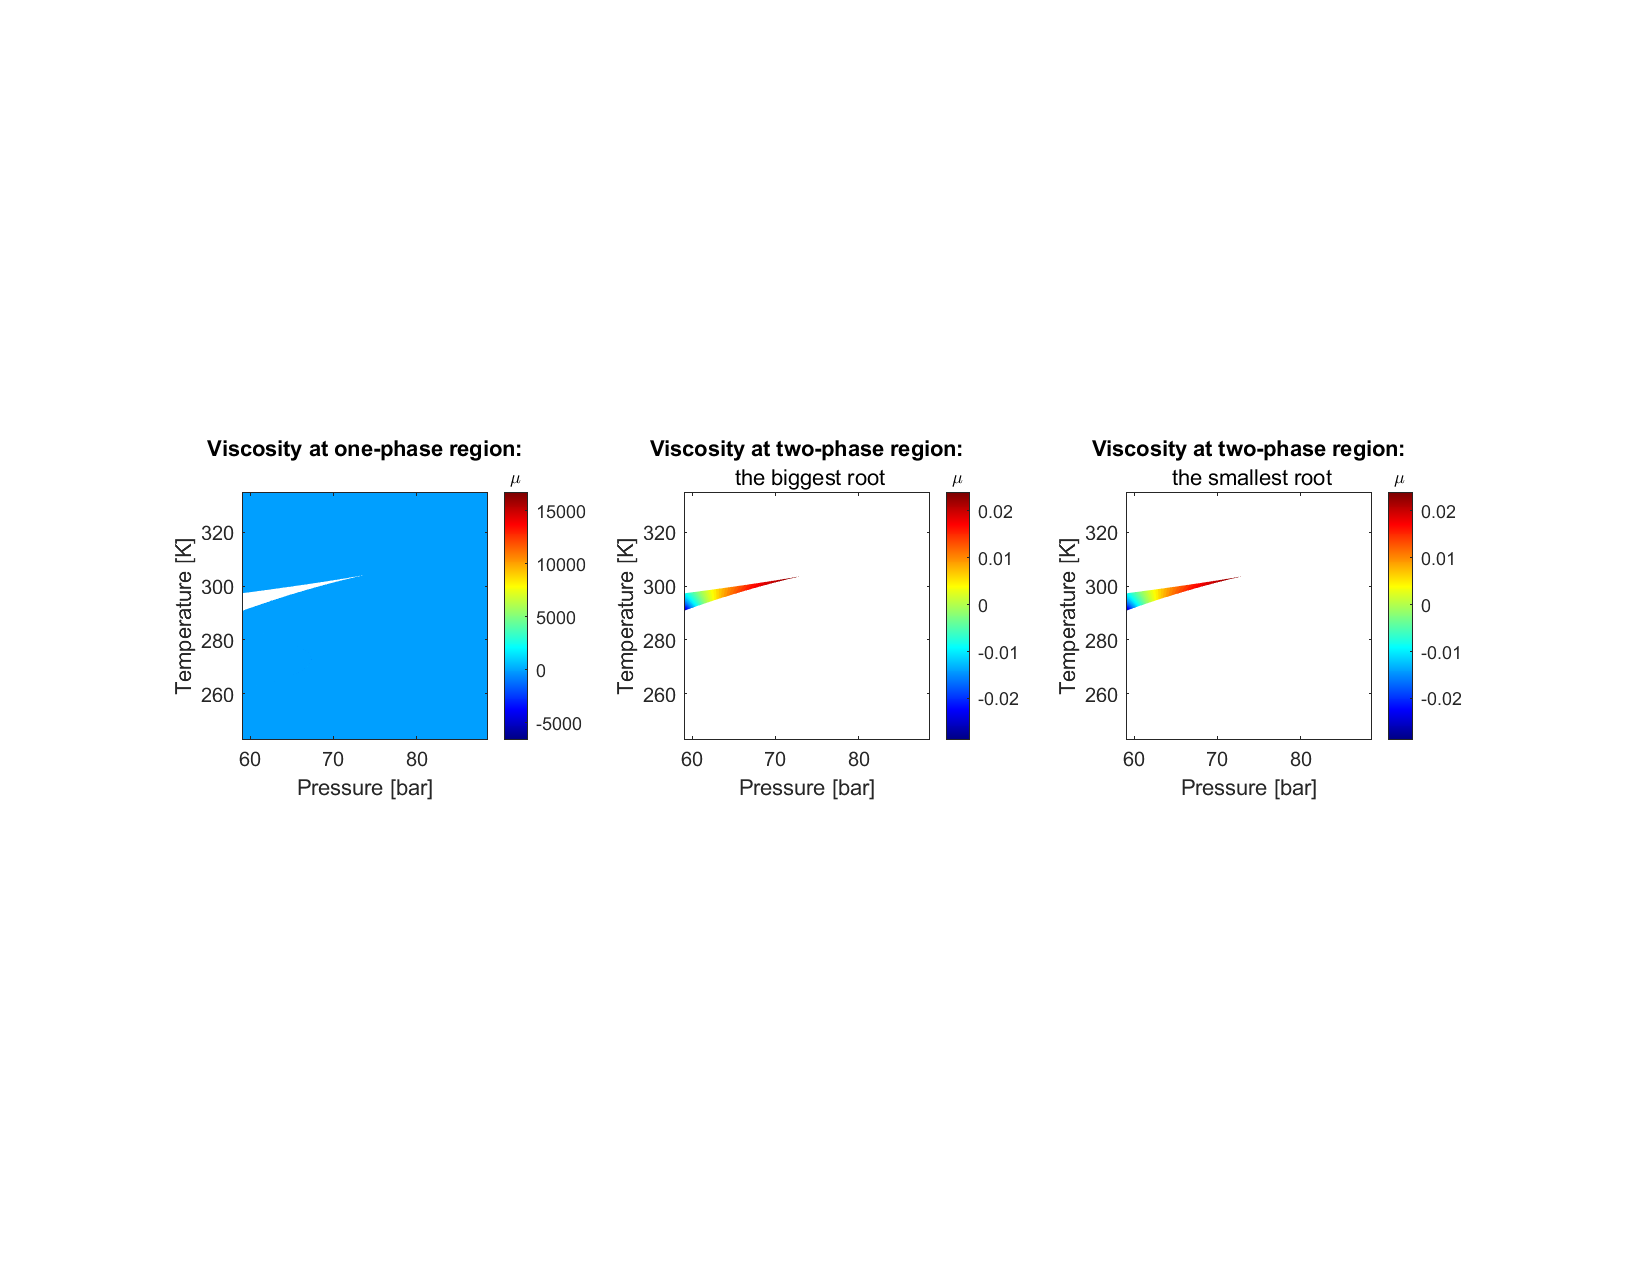
\includegraphics[trim = 1.5cm 11.5cm 2.5cm 10.0cm,clip,width=\textwidth]{Figures/MU.pdf}	
		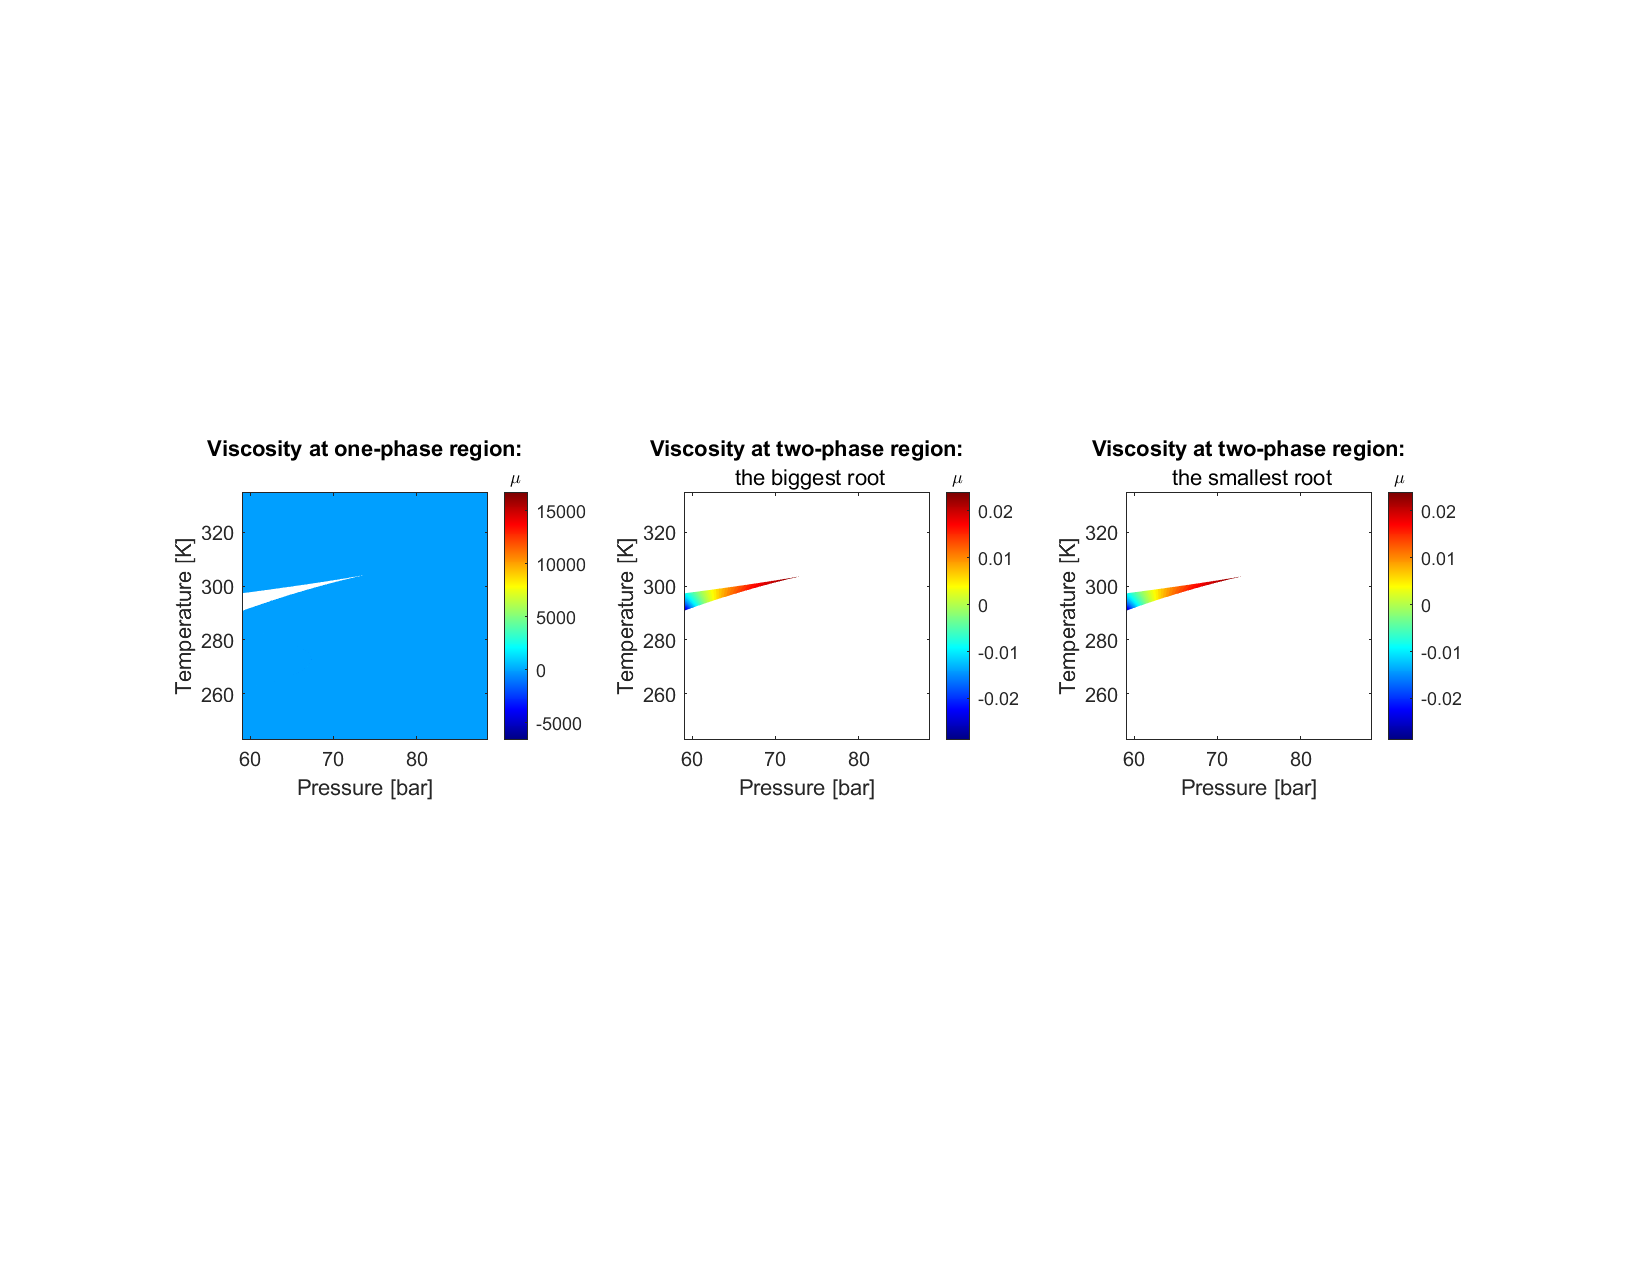
\includegraphics[trim = 1.5cm 4.0cm 2.5cm 19.0cm,clip,width=\textwidth]{Figures/MU.pdf}	
		\caption{Viscosity obtained based on different correlations } 
		\label{fig: SFE_Properties_mu}
	\end{figure*} 
	
	Similarly, several correlations for thermal conductivity of $CO_2$ were compared in Figure \ref{fig: SFE_Properties_kt}. The presented figures show regions around the critical point where the singularity is present. Similarities between specific heat and thermal conductivity can be observed. The NIST correlation (\citet{Huber2016}) captures the singular behaviour of thermal conductivity around the critical point. The correlations are applicable for the temperature range from the triple point to 1100 $K$ and pressures up to 200 $MPa$. 
	
	\begin{figure*}[H]
		\centering
		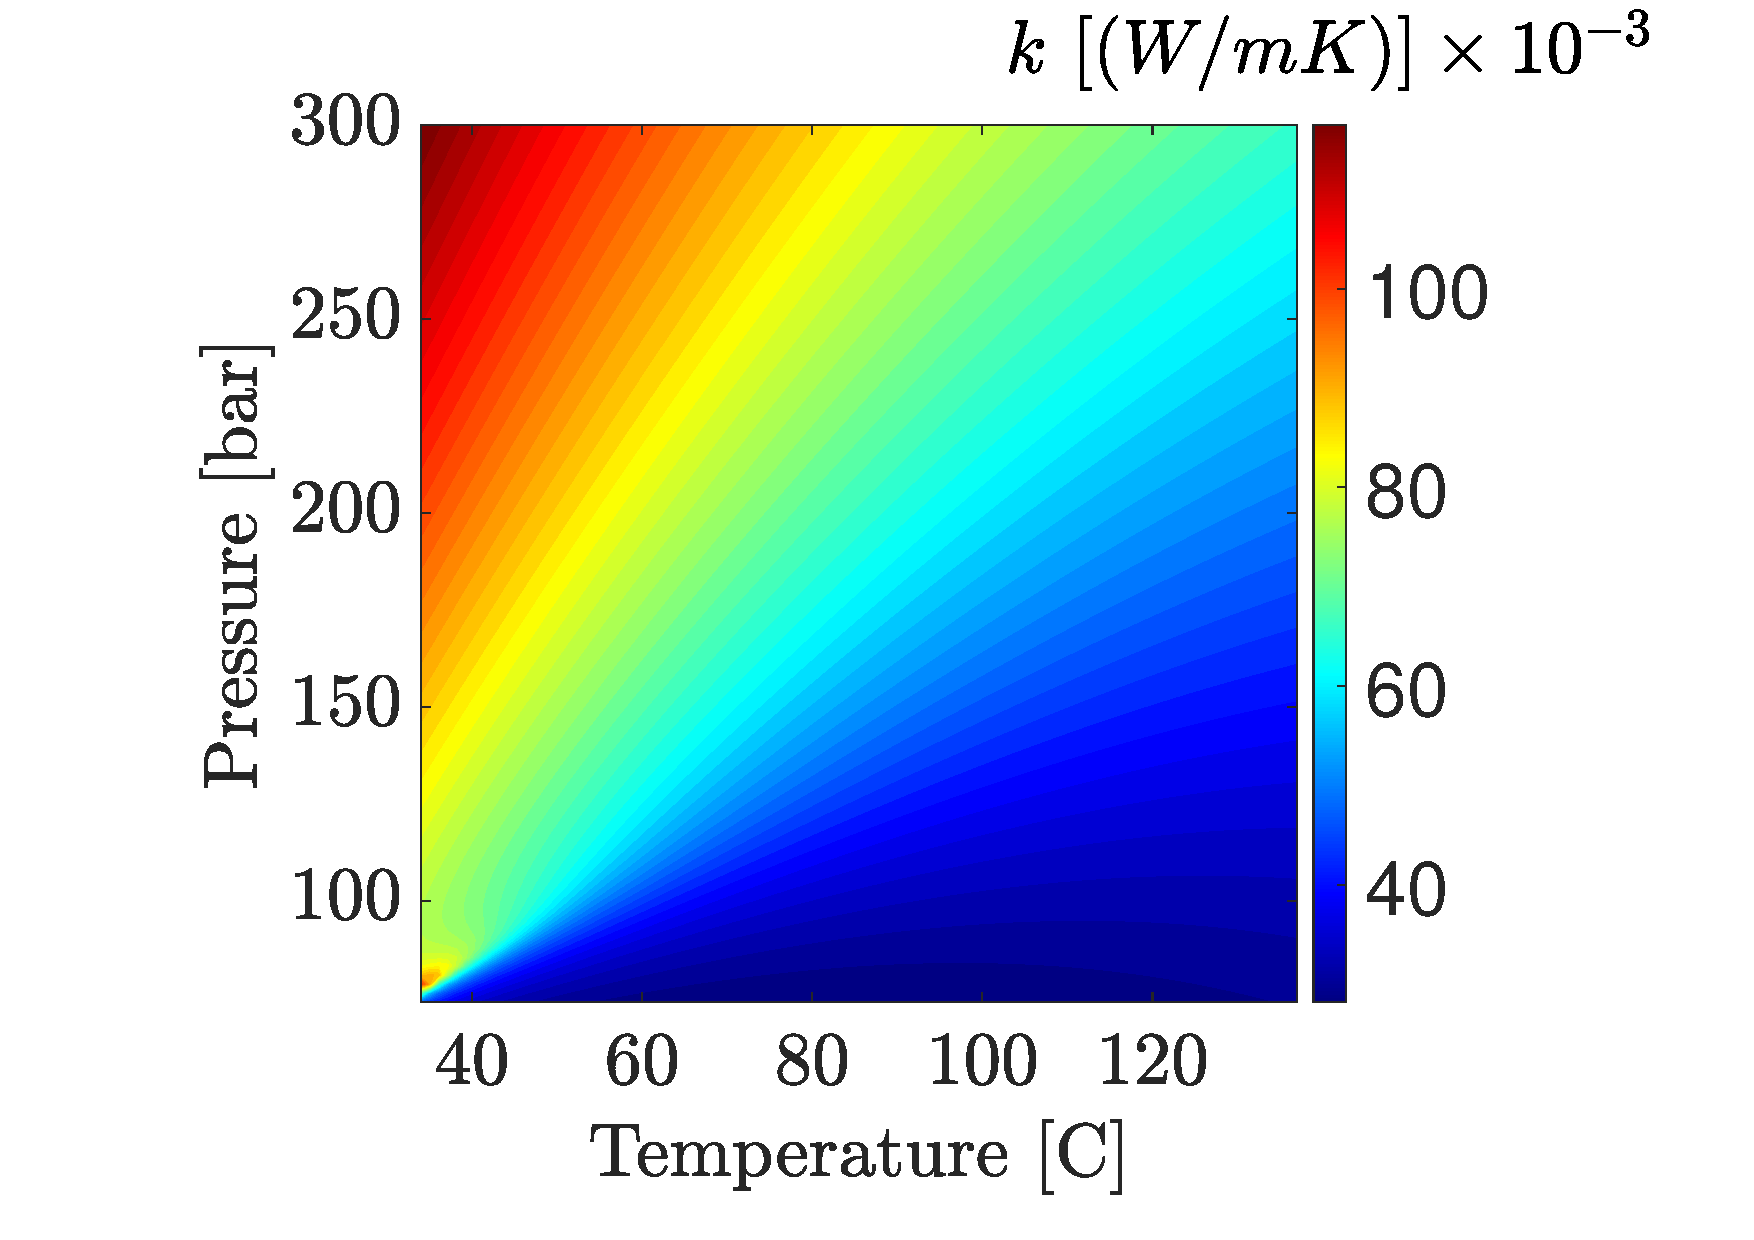
\includegraphics[trim = 1.5cm 2.5cm 1.5cm 2.0cm,clip,width=0.95\textwidth]{Figures/KT.pdf}	
		\caption{Thermal conductivity obtained based on different correlations }
		\label{fig: SFE_Properties_kt}
	\end{figure*} 
	
\end{document}